\section{Shell Elements}
Mathematical fundamentals of shell elements divided into the two parts and the coordinate transformation
 \subsection{Introduction to Linear Elasticity Problems}
 - \cite{steinke2005finite} ch3.1 (S.61)\newline
 - Einführung von Vektoren und Matrizen (Verschiebungsvektor, Tensoren bzw. Vektoren der Dehnungen und Spannungen)\newline
 - Verknüpfung der Versch. mit den Dehnungen + Stoffgesetz (kinematische Beziehung)\newline
 - ???
 
 In the following the fundamental equations of linear elasticity will be considered. Here, the spatial case is used for demonstration, but every lower dimensional problem can easily be derived from it.
 The following definitions will be used in this thesis:
 \begin{equation}
 \vec{u}^T = \left(u\ v\ w\right)\ \mathrm{displacement\ vector}
 \end{equation}
 \begin{equation}
 \vec{f}^T = \left(f_x\ f_y\ f_z\right)\ \mathrm{external\ force\ vector}
 \end{equation}
 The strains and stresses can either be described in form of tensors $\underline{\epsilon}$ and $\underline{\sigma}$, or as vectors $\vec{\epsilon}$ and $\vec{\sigma}$:
 \begin{equation}
 \underline{\epsilon} = \begin{pmatrix}
 \epsilon_{xx} & \epsilon_{xy} & \epsilon_{xz} \\
 \epsilon_{yx} & \epsilon_{yy} & \epsilon_{yz} \\
 \epsilon_{zx} & \epsilon_{zy} & \epsilon_{zz} \end{pmatrix};
 \underline{\sigma} = \begin{pmatrix}
 \sigma_{xx} & \sigma_{xy} & \sigma_{xz} \\
 \sigma_{yx} & \sigma_{yy} & \sigma_{yz} \\
 \sigma_{zx} & \sigma_{zy} & \sigma_{zz} \end{pmatrix}
 \end{equation}
 \begin{equation}
 \vec{\epsilon}^T = \begin{pmatrix}
 \epsilon_{xx} & \epsilon_{yy} & \epsilon_{zz} & 2\epsilon_{xy} & 2\epsilon_{yz} & 2\epsilon_{zx} \end{pmatrix};
 \vec{\sigma}^T = \begin{pmatrix}
 \sigma_{xx} & \sigma_{yy} & \sigma_{zz} & \sigma_{xy} & \sigma_{yz} & \sigma_{zx} \end{pmatrix}
 \end{equation}
 As stated in \cite{steinke2005finite} the relation between displacements and strains is as follows:
 \begin{equation}\label{eq:displ_strain_relation}
 \underline{\epsilon} = \frac{1}{2}\left(\nabla\vec{u} + \vec{u}\:\nabla \right);\quad \vec{\epsilon}
 %= \begin{pmatrix}
 %\frac{\partial}{\partial x} & 0 \\
 %0 & \frac{\partial}{\partial y} \\
 %\frac{\partial}{\partial y} & \frac{\partial}{\partial x} \end{pmatrix} \vec{u}
 = \underline{L}\vec{u}
 \end{equation}
 Equation \ref{eq:displ_strain_relation} relates the displacement vector field $\vec{u}$ with the strain field $\underline{\epsilon}$, or $\vec{\epsilon}$ respectively. Here, $\underline{L}$ is a differential operator. This strain-displacement relation is also called \textit{kinematic relationship} \cite{steinke2005finite}.\\
 In general initial strains can exist inside the material for example due to temperature changes or shrinkage. Such initial strains are denoted $\vec{\epsilon_0}$ and the stresses will be influenced by the difference between the actual and initial strains. Additionally one could imagine initial residual stresses $\vec{\sigma_0}$ that can be added to the general equation:
 \begin{equation}\label{eq:stress-strain-relation}
 \vec{\sigma} = \underline{D}\left(\vec{\epsilon}-\vec{\epsilon_0}\right)+\vec{\sigma_0},
 \end{equation}
 where $\underline{D}$ is the material matrix. In the simplest case of linear elasticity with isotropy, $\underline{D}$ only contains two parameters, namely the elastic modulus $E$ (also known as the Young's modulus) and the Poisson's ratio $\nu$. The former one defines the relationship between the stress and strain in a material, the latter one results as the quotient of the fraction of expansion and the fraction of compression for small changes.
 In the following the initial conditions are ignored, resulting in the a simpler form of equation \ref{eq:stress-strain-relation}:
 \begin{equation}
 \vec{\sigma} = \underline{D}\ \vec{\epsilon}
 \end{equation}
 For the said isotropic case $\underline{D}$ results in \cite{zienkiewicz2000finite}:
 \begin{equation}
 \underline{D} = \frac{E}{1-\nu^2}\begin{pmatrix}
 1 & \nu & 0 \\
 \nu & 1 & 0 \\
 0 & 0 & \frac{1-\nu}{2}
 \end{pmatrix}
 \end{equation}
 \subsection{Plane Element}
 First part of shell element: plane part. derivation of this part with two exemplary finite element types
  \subsubsection{Problem Definition}\label{sec:PlaneProbDef}
  %- Bild ähnlich ch7.1 mit xy-Ausdehnung, Dicke t, Mittelfläche, Rand, KoSys; Streckenlast q0 und Volumenkraft g aber weglassen\newline
  \begin{figure}
\centering
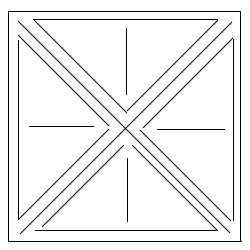
\includegraphics[width=0.7\linewidth]{figures/platzhalter}
\caption[kurze Unter-Überschrift]{lange Unter-Überschrift}
\label{fig:platzhalter}
\end{figure}
  In figure \ref{fig:platzhalter} an object is shown which extends to the x and y axis as its primary direction. The extend in z-direction is smaller and denoted by thickness $t$. The mid place located in between the top and bottom surface areas has the coordinate $z=0$. Its local z-axis equals the normal vector of the mid place. Such an object is called \textit{plane} in the following.
  
  %- Bed. für ebenen Spannungszustand (eb. Dehnungszustand erwähnen und auf Ref (z.B. Zienkiewicz) verweisen)\newline
  There are two different problem definitions regarding plane elements: Plane stress and plane strain. The directions of displacements $u$ and $v$ along the orthogonal local x and y axis defining its displacement field is a common feature of both problems. Also, both have in common, that only strains and stresses in the xy plane have to be considered: Instead of nine, only three components remain. While in the case of plane stress all other stress components are zero, in plane strain the stress in direction perpendicular to the xy plane is non-zero. In this thesis only plane stress will be discussed in further detail. More information about plane strain is given in \cite{zienkiewicz2000finite}. %TODO weitere referenz mit details dazu
  The following conditions must be satisfied such that a plane can be in \textit{plane stress} \cite{steinke2005finite}:
  \begin{itemize}
  	\item The thickness $t$ varies only slightly and it must hold: $t/l \ll 1$, with $l$ the extent of the larger side of the plane element.
  	\item The load is applied to the mid place.
  	\item Displacements, strains and stresses are constant across the thickness.
  \end{itemize}
  The stress components $\sigma_{xz},\sigma_{yz},\sigma_{zz}$ normal to the surface areas with $z \pm t/2$ vanish (equals zero). Therefore only the two normal stress components $\sigma_{xx}$ and $\sigma_{yy}$ and the transverse stress component $\sigma_{xy}$ are left non-zero.
    
  %- Verschiebungen, Dehnungen und Spannungen beschreiben + kinematische Beziehung + Stoffgleichung\newline
  Displacements can only occur in x and y direction. $u$ will be the displacement along x and $v$ along y. The displacement field $\vec{u}$ is as follows:
  \begin{equation}
  \vec{u}=\begin{pmatrix}
  u(x,y) & v(x,y)
  \end{pmatrix}^T
  \end{equation}
  The vector for the strain components:
  \begin{equation}
  \vec{\epsilon}=\begin{pmatrix}
  \epsilon_{xx} & \epsilon_{yy} & 2\epsilon_{xy}
  \end{pmatrix}^T
  \end{equation}
  Sometimes $2\epsilon_{xy}$ is shortened to $\gamma_{xy}$ \cite{steinke2005finite}.
  The vector holding the stress components is similar to that of the strain's vector:
  \begin{equation}
  \vec{\sigma}=\begin{pmatrix}
  \sigma_{xx} & \sigma_{yy} & \sigma_{xy}
  \end{pmatrix}^T
  \end{equation}
  The kinematic relationship $\vec{\epsilon}=\underline{L}\vec{u}$ \ref{eq:displ_strain_relation} linking the displacements $\vec{u}$ with the strains $\vec{\epsilon}$ at full length:
  \begin{equation}\label{eq:t3displ-str-rel}
  \vec{\epsilon} = \begin{pmatrix}
  \epsilon_{xx} \\
  \epsilon_{yy} \\
  2\epsilon_{xy}
  \end{pmatrix} =
  \begin{pmatrix}
  \frac{\partial u}{\partial x} \\
  \frac{\partial v}{\partial y} \\
  \frac{\partial u}{\partial y} + \frac{\partial v}{\partial x}
  \end{pmatrix} =
  \begin{pmatrix}
  \frac{\partial}{\partial x} & 0 \\
  0 & \frac{\partial}{\partial y} \\
  \frac{\partial}{\partial y} & \frac{\partial}{\partial x}
  \end{pmatrix}
  \begin{pmatrix}
  u \\
  v
  \end{pmatrix}
  = \underline{L} \vec{u}
  \end{equation}
  With the strains known and considering equation \ref{eq:displ_strain_relation} one can calculate the stresses $\vec{\sigma}$:
  \begin{equation}\label{eq:sigma=D*eps}
  \vec{\sigma} = \begin{pmatrix}
  \sigma_{xx} \\
  \sigma_{yy} \\
  \sigma_{xy}
  \end{pmatrix} = \frac{E}{1-\nu^2} \begin{pmatrix}
  1 & \nu & 0 \\
  \nu & 1 & 0 \\
  0 & 0 & \frac{1-\nu}{2}
  \end{pmatrix} \begin{pmatrix}
  \epsilon_{xx} \\
  \epsilon_{yy} \\
  2\epsilon_{xy}
  \end{pmatrix} = \underline{D} \vec{\epsilon} = \underline{D}\; \underline{L} \vec{u}
  \end{equation}
  %- Randbedingungen: q0 Streckenlast beschreiben, aber angeben, dass sie hier nicht beachtet werden, punktf. Ladungen werden hier benutzt\newline
  % TODO hier fehlt der Abschnitt über die Randbedingungen steinke s. 214(227)
  natural boundary conditions in form of nodal forces: $\vec{F} = \begin{pmatrix}
  F_x & F_y
  \end{pmatrix}^T$
  
  %- resultierendes Gesamtpotential ohne b und q
  % TODO pi-potenzial einführen
  The total potential of the plane element problem looks as follows:
  \begin{equation}\label{eq:planeFunctional}
  \Pi = 1/2 \int_{V}\vec{\epsilon}^T\vec{\sigma}dV - \vec{u}^T \vec{F},
  \end{equation}
  with the first term being the elastic strain energy and the second term the single forces.
  
  \subsubsection{Tri-3 Plane Element}
  mathematical derivation of three node triangular plane element \textbf{discretization}\\
  see Steinke \cite{steinke2005finite} page 215-221\\
  % Bild von trianguliertem Körper\\
  \begin{figure}
  	\centering
  	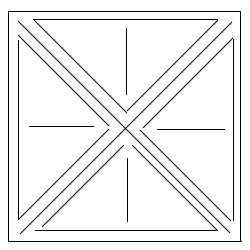
\includegraphics[width=0.7\linewidth]{figures/platzhalter}
  	\caption[kurze Unter-Überschrift]{lange Unter-Überschrift}
  	\label{fig:platzhalter}
  \end{figure}
  In section \ref{sec:PlaneProbDef} the plane's functional was derived. Now the focus is on the functional's discretization. Figure \ref{fig:platzhalter} shows a general, planar object defined to be placed in the xy-plane. The first discretization step is to divide the object into single triangles approximating the shape of it. This process is called triangulation. Every one of these triangles then represents a finite element with one node at every corner. The finer the triangulation is done the better the object and its boundary are matched by its discrete complement, but also the more finite elements have to be considered in later calculations.
  \begin{figure}
  	\centering
  	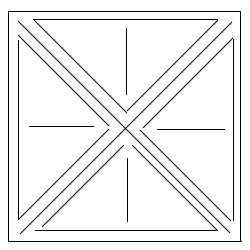
\includegraphics[width=0.7\linewidth]{figures/platzhalter}
  	\caption[kurze Unter-Überschrift]{lange Unter-Überschrift}
  	\label{fig:platzhalter}
  \end{figure}
  One triangular finite element is shown in Figure \ref{fig:platzhalter}. It is defined by the coordinates $(x_i,y_i)$ of its three nodes. Since the element is located in the xy-plane, the z-coordinate is of no interest and will be ignored. At every node, forces can be applied denoted with $F_{x_i}$ and $F_{y_i}$. Accordingly, every node can be displaced. The movement along the x-axis is denoted with $u_i$, or with $v_i$ along the y-axis respectively. Note, that the node numbering is in counter-clockwise direction. This definition will be kept throughout the thesis, and is important to remember when implementing the FEM-code in order to reduce errors.
  In this thesis only triangles defined by three nodes are discussed. There are many more finite elements forming triangles, such as six node triangles or even seven node triangles. The main difference between these types of elements are the order of shape functions. More details about higher order triangular finite elements can be found in %TODO \cite
  
  % ansatzfunktion (abgewandelt statt phi, u und v separat)\\
  In the case of a three node triangle the basis functions for the two displacements $u$ and $v$ are as follows \cite{steinke2005finite}:
  \begin{equation}\label{eq:t3_ansatzU}
  u(x,y) = a_0 + a_1L_1 + a_2L_2 = \begin{pmatrix}
  1 & L_1 & L_2
  \end{pmatrix} \begin{pmatrix}
  a_0 \\ a_1 \\ a_2
  \end{pmatrix} = \vec{x}^T \vec{a},
  \end{equation}
  \begin{equation}\label{eq:t3_ansatzV}
  v(x,y) = a_0 + a_1L_1 + a_2L_2 = \begin{pmatrix}
  1 & L_1 & L_2
  \end{pmatrix} \begin{pmatrix}
  a_0 \\ a_1 \\ a_2
  \end{pmatrix} = \vec{x}^T \vec{a},
  \end{equation}
  both defined in triangular coordinates (see figure \ref{fig:platzhalter}).
  % dreieckskoordinaten (ähnlich bild 2.7 auf s.39(53))
  \begin{figure}
  	\centering
  	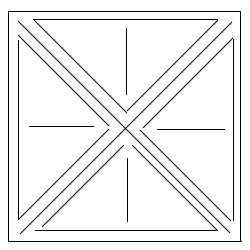
\includegraphics[width=0.7\linewidth]{figures/platzhalter}
  	\caption[kurze Unter-Überschrift]{lange Unter-Überschrift}
  	\label{fig:platzhalter}
  \end{figure}
  % interpolationsbedingunen führen auf Formfunktionen\\
  To get the unknown coefficients $a_i$, values for the triangular coordinates are set. This creates a system of linear equations:
  \begin{align}
  u(L_1=1, L_2=0) = u_1 &\rightarrow u_1 = a_0 + a_1 \nonumber\\
  u(L_1=0, L_2=1) = u_2 &\rightarrow u_2 = a_0 + a_2 \nonumber\\
  u(L_1=0, L_2=0) = u_3 &\rightarrow u_3 = a_0
  \end{align}
  Alternatively, this could be also done with $v$. Written as matrix and vector:
  \begin{align}
  \underline{A} \vec{a} = \vec{u} \nonumber\\
  \begin{pmatrix}
  1 & 1 & 0\\
  1 & 0 & 1\\
  1 & 0 & 0
  \end{pmatrix} \begin{pmatrix}
  a_0 \\ a_1 \\ a_2
  \end{pmatrix} = \begin{pmatrix}
  u_1 \\ u_2 \\ u_3
  \end{pmatrix}
  \end{align}
  Now, inverting matrix $A$ the coefficients can be found:
  \begin{equation}\label{eq:t3_coeffsA}
  \vec{a} = \underline{A}^{-1} \vec{u} = \begin{pmatrix}
  0 & 0 & 1\\
  1 & 0 & -1\\
  0 & 1 & -1
  \end{pmatrix} \begin{pmatrix}
  u_1 \\ u_2 \\ u_3
  \end{pmatrix}
  \end{equation}
  If one put equation \ref{eq:t3_coeffsA} into \ref{eq:t3_ansatzU}, or the analogon into \ref{eq:t3_ansatzV}, the shape functions for the three node triangular finite element will be derived, as described in \cite{steinke2005finite}:
  \begin{align}\label{eq:t3SF}
  u &= \vec{x}^T \vec{a} = \vec{x}^T \underline{A}^{-1}\vec{u} = \vec{N}^T\vec{u} \nonumber\\
  \vec{N}^T &= \vec{x}^T \underline{A}^{-1} =
  \begin{pmatrix}
  1 & L_1 & L_2
  \end{pmatrix} \begin{pmatrix}
  0 & 0 & 1\\
  1 & 0 & -1\\
  0 & 1 & -1
  \end{pmatrix} \nonumber\\
  &= \begin{pmatrix}
  L_1 & L_2 & 1-L_1-L_2
  \end{pmatrix} = \begin{pmatrix}
  N_1 & N_2 & N_3
  \end{pmatrix}
  \end{align}
  Characteristically for the shape function, as stated in \cite{steinke2005finite}, is, that shape function $N_i$ gets the value 1 at node $i$ and 0 at the two other nodes. The functions are linear with respect to $L_1$ and $L_2$ which can be noticed in equation \ref{eq:t3SF}. As stated before, these shape functions are the same for displacement $u$ and $v$. With the knowledge of the displacement values of the element's nodes one can formulate the displacement functions in triangular coordinate notation as follows:
  \begin{align}
  u &= N_1 u_1 + N_2 u_2 + N_3 u_3 \nonumber\\
  v &= N_1 v_1 + N_2 v_2 + N_3 v_3
  \end{align}
  Or in matrix form:
  \begin{align} \label{eq:t3u=Nu}
  \vec{\tilde{u}} &= \underline{N} \vec{u} \nonumber\\
  \begin{pmatrix}
  u \\ v
  \end{pmatrix} &= \begin{pmatrix}
  N_1 & 0 & N_2 & 0 & N_3 & 0 \\
  0 & N_1 & 0 & N_2 & 0 & N_3
  \end{pmatrix} \begin{pmatrix}
  u_1 \\ v_1 \\ u_2 \\ v_2 \\ u_3 \\ v_3
  \end{pmatrix}
  \end{align}
  The vector $\vec{\tilde{u}}$ describes the element's displacements as product of matrix $\underline{N}$ containing the shape functions and vector $\vec{u}$ containing the displacements of the single triangle's nodes. Now, one can put equation \ref{eq:t3u=Nu} into \ref{eq:t3displ-str-rel}:
  \begin{equation}\label{eq:t3eps=Bu}
  \vec{\epsilon} = \underline{L}\vec{\tilde{u}} = \underline{L}\;\underline{N} \vec{u} = \underline{B} \vec{u}
  \end{equation}
  The product of $\underline{L}$ and $\underline{N}$ is called \textit{strain-displacement matrix} $\underline{B}$.
  In order to calculate the strain-displacement matrix, one has to assemble the $\underline{L}$ matrix containing the first partial derivatives of the triangular element. With the chain rule applied, the partial derivatives look as follows:
  \begin{align}
  \frac{\partial}{\partial L_1} = \frac{\partial x}{\partial L_1} \frac{\partial}{\partial x} + \frac{\partial y}{\partial L_1} \frac{\partial}{\partial y} \nonumber\\
  \frac{\partial}{\partial L_2} = \frac{\partial x}{\partial L_2} \frac{\partial}{\partial x} + \frac{\partial y}{\partial L_2} \frac{\partial}{\partial y}
  \end{align}
  or in matrix notation:
  \begin{align}\label{eq:t3NablaTilde}
  \tilde{\nabla} &= \underline{J} \nabla \nonumber\\
  \begin{pmatrix}
  \frac{\partial}{\partial L_1}\\ \frac{\partial}{\partial L_2}
  \end{pmatrix} &= \begin{pmatrix}
  \frac{\partial x}{\partial L_1} & \frac{\partial y}{\partial L_1}\\
  \frac{\partial x}{\partial L_2} & \frac{\partial y}{\partial L_2}
  \end{pmatrix} \begin{pmatrix}
  \frac{\partial}{\partial x}\\ \frac{\partial}{\partial y}
  \end{pmatrix},
  \end{align}
  where $\underline{J}$ represents the Jacobian, $\nabla$ the partial derivatives in Cartesian coordinates and $\tilde{\nabla}$ the partial derivatives in triangular coordinates. To get the derivatives in Cartesian form the upper equation must be multiplied with the inverse Jacobian $\underline{J}^{-1}$:
  \begin{equation}
  \underline{J}^{-1} = \frac{1}{|\underline{J}|} \begin{pmatrix}
  \frac{\partial y}{\partial L_2} & -\frac{\partial y}{\partial L_1} \\
  \frac{-\partial x}{\partial L_2} & \frac{\partial x}{\partial L_1}
  \end{pmatrix}
  \end{equation}
  The conversion between triangular and Cartesian coordinates can be summarized as follows (see Figure \ref{fig:platzhalter} and \cite{steinke2005finite}):
  \begin{align}\label{eq:triCoord<->CartCoord}
  L_1 + L_2 + L_3 &= 1 \rightarrow L_3 = 1-L_1-L_2 \nonumber\\
  x &= x_1L_1 + x_2L_2 + x_3L_3 = (x_1-x_3)L_1 + (x_2-x_3)L2 + x_3\\
  y &= y_1L_1 + y_2L_2 + y_3L_3 = (y_1-y_3)L_1 + (y_2-y_3)L2 + y_3 \nonumber
  \end{align}
  Considering equation \ref{eq:triCoord<->CartCoord} the Jacobian can now be calculated
  \begin{equation}
  J = \begin{pmatrix}
  \frac{\partial x}{\partial L_1} = x_1-x_3 = x_{13} & \frac{\partial y}{\partial L_1} = y_1-y_3 = y_{13}\\
  \frac{\partial x}{\partial L_2} = x_2-x_3 = x_{23} & \frac{\partial y}{\partial L_2} = y_2-y_3 = y_{23}
  \end{pmatrix} = \begin{pmatrix}
  x_{13} & y_{13}\\
  x_{23} & y_{23}
  \end{pmatrix}
  \end{equation}
  and hence the inverse Jacobian:
  \begin{equation}\label{eq:t3invJac}
  \underline{J}^{-1} = \frac{1}{2 A_\triangle} \begin{pmatrix}
  y_{23} & -y_{13}\\
  -x_{23} & x_{13}
  \end{pmatrix}
  \end{equation}
  The determinant of the Jacobian is two times the area of the triangle. With the help of equation \ref{eq:t3invJac}, \ref{eq:t3NablaTilde} can be reorganized
  \begin{equation}
  \nabla = \underline{J}^{-1} \tilde{\nabla}
  \end{equation}
  and this finally yields to the new version of the differential operator $\underline{L}$ \cite{steinke2005finite}:
  \begin{align}
  \underline{L} = \frac{1}{2 A_\triangle} \begin{pmatrix}
  y_{23}\frac{\partial}{\partial L_1} - y_{13}\frac{\partial}{\partial L_2} & 0 \\
  0 & -x_{23}\frac{\partial}{\partial L_1} + x_{13}\frac{\partial}{\partial L_2} \\
  -x_{23}\frac{\partial}{\partial L_1} + x_{13}\frac{\partial}{\partial L_2} & y_{23}\frac{\partial}{\partial L_1} - y_{13}\frac{\partial}{\partial L_2}
  \end{pmatrix}
  \end{align}
  
  % Dehnungs-Verschiebungs-Beziehung -> führt zu B + Spannungs-Verschiebungs-Beziehung\\
  Next, the strain-displacement matrix $\underline{B}$ can be calculated:
  \begin{align}
  \underline{B} &= \underline{L}\; \underline{N} \nonumber\\
  &= \frac{1}{2 A_\triangle} \begin{pmatrix}
  y_{23}\frac{\partial}{\partial L_1} - y_{13}\frac{\partial}{\partial L_2} & 0 \\
  0 & -x_{23}\frac{\partial}{\partial L_1} + x_{13}\frac{\partial}{\partial L_2} \\
  -x_{23}\frac{\partial}{\partial L_1} + x_{13}\frac{\partial}{\partial L_2} & y_{23}\frac{\partial}{\partial L_1} - y_{13}\frac{\partial}{\partial L_2}
  \end{pmatrix} \nonumber\\
  & \quad \begin{pmatrix}
  L_1 & 0 & L_2 & 0 & 1-L_1-L_2 & 0 \\
  0 & L_1 & 0 & L_2 & 0 & 1-L_1-L_2
  \end{pmatrix} \nonumber\\
  &= \frac{1}{2 A_\triangle} \begin{pmatrix}
  y_{23} & 0 & -y_{13} & 0 & y_{12} & 0 \\
  0 & -x_{23} & 0 & x_{13} & 0 & -x_{12} \\
  -x_{23} & y_{23} & x_{13} & -y_{13} & -x_{12} & y_{12}
  \end{pmatrix}
  \end{align}
  
  % Einsetzen in Gesamtpotential + Variation\\
  With $\underline{B}$ known, one can insert equation \ref{eq:t3eps=Bu} into \ref{eq:sigma=D*eps} to get the stresses:
  \begin{equation} \label{eq:t3sigma=DBu}
  \vec{\sigma} = \underline{D}\;\underline{B} \vec{u}
  \end{equation}
  Finally, every term of the plane element's functional \ref{eq:planeFunctional} can be filled with the above discretized terms:
  \begin{align}\label{eq:t3functional}
  \Pi &= \frac{1}{2} \int_{V}\vec{\epsilon}^T\vec{\sigma}\;dV - \vec{u}^T \vec{F} \nonumber\\
      &= \frac{1}{2} \int_{V}\vec{u}^T \underline{B}^T\underline{D}\;\underline{B}\vec{u}\;dV - \vec{u}^T \vec{F} \nonumber\\
      &= \frac{1}{2} \vec{u}^T \int_{V} \underline{B}^T\underline{D}\;\underline{B}\;dV \vec{u}- \vec{u}^T \vec{F} \nonumber\\
      &= \frac{1}{2}\vec{u}^T \underline{K} \vec{u} - \vec{u}^T \vec{F}
  \end{align}
  with $\underline{K}$ the stiffness matrix and $\vec{F}$ the nodal force vector.
  
  % Bestimmung von K kürzen: wichtig ist nur s.221 K = t*int(H*dA,A) mit dV = t*dA
  The variation of the functional \ref{eq:t3functional} is as follows \cite{steinke2005finite}:
  \begin{align}
  \delta\Pi &= \frac{\partial\Pi}{\partial \vec{u}}\delta\vec{u} = 0 \nonumber\\
            &= \frac{1}{2}\delta\vec{u}^T\frac{\partial\vec{u}^T}{\partial\vec{u}^T}\underline{K}\vec{u} + \frac{1}{2}\vec{u}^T\underline{K}\frac{\partial\vec{u}}{\partial\vec{u}}\delta\vec{u} - \delta\vec{u}\frac{\partial\vec{u}^T}{\partial\vec{u}^T}\vec{F} \nonumber\\
            &= \delta\vec{u}^T\left(\underline{K}\vec{u}-\vec{F}\right) = 0
  \end{align}
  In order to satisfy this equation, the term in between the parenthesis must be zero ($\delta\vec{u}^T$ can have arbitrary values). This leads to the equilibrium equation of the triangular plane element as described in \cite{steinke2005finite}:
  \begin{equation}
  \underline{K}\vec{u} = \vec{F}
  \end{equation}
  Since the thickness $t$ of the element is constant per definition, it is $dV = t\;dA$ and therefore the integral of the stiffness matrix changes to:
  \begin{equation}
  \underline{K} = t \int_A \underline{B}^T\underline{D}\;\underline{B}\;dA = t A_\triangle \underline{B}^T\underline{D}\;\underline{B}
  \end{equation}
  \subsubsection{Quad-4 Plane Element}
  - mathematical derivation of four node quadrilateral plane element\newline
  - see Steinke \cite{steinke2005finite} page 237-250 + Cook \cite{cook2002concepts} page 202-208\\
  - isoparametrisches viereckselement (7.5.1) + bild\\
  - bild von original- und bildebene\\
  - eigenschaften der ansatzfunktion + formfunktionen\\
  - verschiebungen von uv mit formfunktionen und u darstellen\\
  - jacobi-matrix aufstellen, inverse und determinante nicht so genau (bzw. einfach, weil J eh nur 2x2 ist)\\
  - dehnungs-verschiebungs-beziehung AUS ANDERER QUELLE, DA IN \cite{steinke2005finite} UNZUFRIEDENSTELLEND BESCHRIEBEN\\
  - stefigkeitsmatrix $K = int_V(B^TDBdV) = t*int_V(B^TDBdA) = t*int_-1^1 int_-1^1(B^TDB|J|dsdr)$ + erwähnen, dass |J| Flächeninhalt angibt (ref finden)
 \subsection{Plate Bending Element}
 Second part of shell element: plate part. derivation of this part with two exemplary finite element types
  \subsubsection{Problem Definition}
  \cite{steinke2005finite} ch8.1\\
  - bild wie bei \ref{sec:MprobDef}\\
  - hier wird die kirchhoff-platten-theorie verwendet\\
  - voraussetzungen der kirchhoff-platte\\
  - größen der platte: durchbiegung w + verdrehungen dw/dx bzw. dw/dy\\
  - dehnungs-verschiebungs-beziehung\\
  - stoffgleichung (krümmungs-momenten-beziehung) -> führt auf Dp und Querkräfte Qx,Qy\\
  - gleichgewichtsbeziehung der platte (p ist flächenlast; näher untersuchen)\\
  - auf verschiedene randbedingungen der platte eingehen\\
  - funktional der platte\\
  - forderungen an plattenelement
  \subsubsection{Tri-3 Plate Element} \cite{steinke2005finite}\cite{specht1988modified}
  - mathematical derivation of three node triangular plane element\newline
  - see Steinke \cite{steinke2005finite} page 275-282 + \cite{specht1988modified} for reference of element\\
  - 8.4.4 beschreibt probleme mit einigen dreiecksplattenelementen, deshalb für meine arbeit element von specht \cite{specht1988modified}\\
  - ansatzfunktion nach specht\\
  - interpolationsbedingungen\\
  - entwicklung der formfunktionen\\
  - krümmungs-verschiebungs-beziehung\\
  - steifigkeitsmatrix
  \subsubsection{Quad-4 Plate Element}
  - mathematical derivation of four node quadrilateral plane element\newline
  - see Zienkiewicz \cite{zienkiewicz2000finite} page 174-177,219-222  \cite{zienkiewicz1977fem} ???  \textbf{\cite{batoz1982evaluation} page 1658-1662}\\
  - formulierung als DKQ element\\
  - \textbf{!! formatierung an meine anpassen, da sehr unterschiedlich zu anderen referenzen !!}\\
  - dkq basiert auf diskretisierung der stress-energie, unter vernachlässigung der transverse shear strain energy (gl.(1) s.4)\\
  - krümmungsvektor, Db angeben\\
  - considerations für dkq formulierung\\
  - formfunktionen, koeffizienten\\
  - jacobi-matrix, -inverse, determinante\\
  - krümmungs-verschiebungs-beziehung\\
  - steifigkeitsmatrix
 \subsection{Coordinate Transformation} %\cite{steinke}
 \textit{erster Entwurf}\newline
 see \cite{nguyen2008smoothed}; genau: \cite{zienkiewicz2000finite}\\
 The nodes and elements in the mesh are defined in global three dimensional space. The elements need to be transformed into local two dimensional space in order to be able to calculate their local stiffness matrix. This local stiffness matrix must then be transformed back into the global system.
 Transform arbitrary 3D triangle onto xy-Plane:
 % Bild von Dreieck mit ABC, globalem KoSys, lokalem KoSys mit Ursprung in A, x-Achse auf Vektor AB usw.\newline
 - given triangle with vertices $A=(a_x, a_y, a_z), B=(b_x, b_y, b_z)$ and $C=(c_x, c_y, c_z)$ ordered in counter-clockwise direction\newline
 - let $U$ be the vector from node $A$ to $B$: $U = B-A = (b_x-a_x, b_y-a_y,b_z-a_z)$ and let $V$ be the vector from node $A$ to $C$: $V = C-A = (c_x-a_x,c_y-a_y,c_z-a_z)$\newline
 - First local unit vector $\tilde{x} = \frac{1}{\left|U\right|}U$\newline
 - Second local unit vector $\tilde{z} = U \times V \longrightarrow \tilde{z} = \frac{1}{\tilde{z}}\tilde{z}$\newline
 - Third local unit vector $\tilde{y} = \tilde{z} \times \tilde{x}$\newline
 - Define transformation matrix $T$ as follows: \[T = \begin{pmatrix}
 \tilde{x}^T\\ \tilde{y}^T\\ \tilde{z}^T
 \end{pmatrix}
 = \begin{pmatrix}
  \tilde{x}_x & \tilde{x}_y & \tilde{x}_z\\ \tilde{y}_x & \tilde{y}_y & \tilde{y}_z\\ \tilde{z}_x & \tilde{z}_y & \tilde{z}_z
  \end{pmatrix}\]
  - Assembly of element's stiffness needs derivatives. Therefore every triangle can be translated in such a way, that node $A$ lies in the global origin.\newline
  - It follows: $\tilde{A} = \left(0\ 0\ 0\right)^T, \tilde{B} = \left(\tilde{b}_x\ 0\ 0\right)^T, \tilde{C} = \left(\tilde{c}_x\ \tilde{c}_y\ 0\right)^T$\newline
  - Node $A$ will not be changed by the transformation with $T$, $B$ will be projected onto the local x-axis due to the definition of it as the vector between $A$ and $B$ and $C$ will be projected onto the local $xy$-plane.\newline
  - One can see that the z component vanishes by transforming into local space\newline
  \newline
  % Bild von bel. Viereck mit ABCD, IJKL, globalem KoSys, lokalem KoSys mit Ursprung auf Schnittpunkt der gestrichelten Linien von JL und IK\newline
  - given quadrilateral with vertices $A=(a_x, a_y, a_z), B=(b_x,b_y,b_z), C=(c_x,c_y,c_z), D=(d_x,d_y,d_z)$ ordered in counter-clockwise direction\newline
  - let $I$ be the midpoint of the edge $AB$ as follows: $I = A+\frac{1}{2}(B-A)$. Analogously let $J$,$K$ and $L$ be the midpoints of the edges $BC$, $CD$ and $DA$: $J = B+\frac{1}{2}(C-B), K = C+\frac{1}{2}(D-C), L = D+\frac{1}{2}(A-D)$\newline
  - let $U$ be the vector from node $L$ to $J$: $U = J-L = (j_x-l_x,j_y-l_y,j_z-l_z)$ and let $V$ be the vector from node $I$ to $K$: $V = K-I = (k_x-i_x,k_y-i_y,k_z-i_z)$\newline
  - First local unit vector $\tilde{x} = \frac{1}{\left\|U\right|}U$\newline
  - Second local unit vector $\tilde{z} = U \times V \longrightarrow \tilde{z} = \frac{1}{\left|\tilde{z}\right|}\tilde{z}$\newline
  - Third local unit vector $\tilde{y} = \tilde{z} \times \tilde{x}$\newline
  - Define transformation matrix $T$ as follows: \[T = \begin{pmatrix}
   \tilde{x}^T\\ \tilde{y}^T\\ \tilde{z}^T
   \end{pmatrix}
   = \begin{pmatrix}
    \tilde{x}_x & \tilde{x}_y & \tilde{x}_z\\ \tilde{y}_x & \tilde{y}_y & \tilde{y}_z\\ \tilde{z}_x & \tilde{z}_y & \tilde{z}_z
    \end{pmatrix}
    \]
 \subsection{Shell Element}
 The combination of the two previous parts and the transformations results in the final shell element\newline
 - bild wie bei 8.7 von scheibe und platte und kombination zu schale + erklärungen, welche unbekannten und kräfte man bei welchem teil hat\\
 - erklärung, warum man hier einfach Plane und Plate unabhängig voneinander berechnen und dann zusammenwerfen darf\\
 - gesamtsteifigkeitsmatrix besteht aus blöcken (3x3 bei tri3, 4x4 bei quad4), Ku=F (gleichung 718 bei \cite{steinke2005finite})
 - Sei $K_m$ die lokale Steifigkeitsmatrix vom Membran/Plane-Teil und $K_p$ die vom Plate-bending-Teil\\
 - Kij weisst in der Spalte theta\_z und Zeile theta\_z $(k_ij)_66$ eine null auf -> erklärung und warum schlecht. ANDERE REFERENZ ERKLÄRT, WAS WIR DESHALB MACHEN (1/1000 der diagonalwerte)\\
 - Dann muss die (Rück-)Transformationsmatrix $T$ erstellt werden, da SKM im lokalen KoSys definiert ist, aber in die globale Systemmatrix einsortiert werden muss\\
 - Je nachdem ob 3 oder 4 Knotenelement (Tri-3/Quad-4) sieht $K$ und $T$ natürlich anders aus\newline
 - Wir transformieren blockweise von lokal nach global zurück ($K_{ij}, 1 \leq i,j \leq 3(4)$)\newline
 \newpage